% 中文摘要      I_chabstract.tex
% 英文摘要      II_enabstract.tex
% 誌謝          III_acknowledge.tex

% 主程ot                00_masterthesis.tex
% 緒論                  01_introduction.tex
% 背景知識與相關文獻    02_relatedwork.tex
% 問題分析              03_analysis
% 研究方法              04_method.tex
% 實驗與結果分析        05_experiment.tex
% 結論                  06_conclusion.tex
% 附錄                  07_appendix.tex

% clean.bat 為清除、複製檔案於 C:\xtemp 使用。
% IEEEtran.sty 為文獻格式必須檔。
% *.bib 為文獻檔
%%%%%%%%%%%%%%%%%%%%%%%%%%%%%%%%%%%%%%%%%%%%%%%%%%%%%%%%%%%%%%%%%%%%%%%%%%%%%%%%%%%%%%%%%%%%%%%%%%%%
\documentclass[12pt,oneside,openany,a4paper,draft=FALSE]{book}

% 套件集
%\usepackage[left=3cm,top=3cm,nohead]{geometry}
%\usepackage[total={15cm,24cm}, top=35mm, left=36mm, includefoot]{geometry}
\usepackage[total={15cm,24cm}, top=30mm, left=30mm, includefoot]{geometry}  %版面格式

%首行縮排
\usepackage{indentfirst}
\usepackage{times}
\usepackage{titlesec}
\usepackage{caption}
\usepackage{comment}
\usepackage{bm}
%\usepackage[usenames,dvipsnames]{color}     %自訂文字顏色
\usepackage{graphicx,subfigure,float}       % 所有圖片均為浮動狀態,可為圖片編碼
\usepackage{tikz}
\usepackage{amsmath,amssymb}                % 數學式
%\usepackage{color,colortbl,lettrine,wrapfig}
%\usepackage{epstopdf} %EPS轉PDF功能
%\usepackage[bookmarks=false,colorlinks=true,breaklinks=true]{hyperref} %PDF書籤與連結功能
\usepackage[numbered]{bookmark} %PDF書籤與連結功能
\usepackage[titletoc]{appendix}
%\usepackage{breakurl}

%註腳不縮排
\usepackage[bottom,hang,flushmargin]{footmisc}

% 文獻套件
\usepackage[square,numbers]{natbib} %中英文文獻
%\usepackage{natbib}
\usepackage{bibentry}
%\usepackage{biblatex}
%\usepackage[notocbib]{apacite}     % use APA citation
%\usepackage{IEEEtran}   %IEEE文獻
\usepackage[notindex,nottoc,notlot,notlof]{tocbibind}

\usepackage{longtable}
\usepackage{url}
\usepackage{wallpaper}     % 浮水印
% 引入pdf
\usepackage{pdfpages}
% 表格套件
\usepackage{array}
\usepackage{fancyhdr}
\usepackage{rotating}   % 旋轉表格,將某頁版面由直排轉為橫排,適合用於旋轉占滿一頁的表格或圖形
\usepackage{booktabs}
%\usepackage{graphicx,floatrow}

% 數學
\usepackage{amsthm}     % 排版數學文稿的定理與定義
\usepackage{amsmath}
\usepackage{enumerate}  % 條列項目 (阿拉伯數字編號)

%% 中文專用
\usepackage{fontspec} %加這個就可以設定字體
\usepackage{xeCJK} %讓中英文字體分開設置

\usepackage{mathptmx}
\usepackage[T1]{fontenc}


%畫圖套件
\usepackage{mathrsfs}
\usepackage{pgfplots}
\pgfplotsset{compat=1.15}
\usetikzlibrary{arrows}

%-----

% 設定『目錄』名稱
\renewcommand{\contentsname}{目錄}
\renewcommand{\listfigurename}{圖目錄}
\renewcommand{\listtablename}{表目錄}
%\renewcommand{\appendixtocname}{附錄}   % if \appendix  is used.
\renewcommand{\appendixname}{附錄}   % if \appendix  is used.
\renewcommand{\tablename}{表}
\renewcommand{\figurename}{圖}
\renewcommand{\bibname}{參考文獻}

\hypersetup{
    bookmarks=true,         % show bookmarks bar?
    colorlinks=true,        % false: boxed links; true: colored links
    linkcolor=black,          % color of internal links (change box color with linkbordercolor)
    citecolor=black,          % color of links to bibliography
    filecolor=cyan,         % color of file links
    urlcolor=magenta        % color of external links
}

%\newcommand{\img}{C:/Dropbox/ntpu_thesis/plot/}%如果所有圖檔存放在其他地方,先定義位置

\pagestyle{fancy}
\fancyhf{}
\renewcommand{\chaptermark}[1]{\markboth{\thechapter .\ #1}{}}  % 去除章編號前後的字
\titleformat{\chapter}[display]{\center\LARGE\sf}{第\ \thechapter\ 章}{0.2cm}{}  %設計章節標題式樣,標題置中
\titlespacing{\chapter}{0pt}{-50pt}{25pt}   %設計章節標題式樣,控制間距
%\fancyhead[RO,RE]{\leftmark}   %章節標題於頁眉/頁足上
\fancyfoot[CO,CE]{\thepage}

\renewcommand{\headrulewidth}{0pt}  % 頁眉下方的橫線
%\renewcommand{\footrulewidth}{0pt} % 設定頁首多一條粗細是 0.4 pt 的水平線

% 設定itemize符號
\renewcommand{\labelitemi}{$\bullet$}
\renewcommand{\labelitemii}{$\circ$}

%設定英文字型,不設的話就會使用預設的字型
\setmainfont{Times New Roman}

% 設定中文字體
\setCJKmainfont{標楷體} %設定中文為系統上的字型,而英文不去更動,使用原TeX字型
%\setCJKmainfont{cwTeXKai}
\XeTeXlinebreaklocale "zh"
\XeTeXlinebreakskip = 0pt plus 1pt %這兩行一定要加,中文才能自動換行


\renewcommand{\baselinestretch}{1.25}   %依照文章預設行距增加為 1.25倍(不同字型大小行距值,加大為1.25倍)

% 以下是目錄章節後面打點格式的設定:http://vardesa.blog.hexun.com.tw/58537832_d.html
\makeatletter
\def\@bfdottedtocline#1#2#3#4#5{%
\ifnum #1>\c@tocdepth \else
\vskip \z@ \@plus.2\p@
{\leftskip #2\relax \rightskip \@tocrmarg \parfillskip -\rightskip
\parindent #2\relax\@afterindenttrue
\interlinepenalty\@M
\leavevmode \bfseries
\@tempdima #3\relax
\advance\leftskip \@tempdima \null\nobreak\hskip -\leftskip
{#4}\normalfont\nobreak
\leaders\hbox{$\m@th
\mkern \@dotsep mu\hbox{.}\mkern \@dotsep
mu$}\hfill
\nobreak
\hb@xt@\@pnumwidth{\hfil\normalfont \normalcolor #5}%
\par}%
\fi}
\renewcommand*\l@chapter{\@bfdottedtocline{0}{0em}{1.5em}}
\makeatother

% 定義『各章節標題、圖表、頁尾註記』字型

\theoremstyle{plain}   % 排版格式,{plain}:最醒目格式
\newtheorem{thm}{定理}  % 將 Theorem 改為國字「定理」
\newtheorem{thmm}{定義}


%
%   調整內縮長度(依據學校規定與不同版面、字型調整)
%
\parindent=0.85cm
%% 修改中文標題與格式定義
\date{2013.9.18}    %版本日期

%%%%% 論文開始 %%%%%
\begin{document}

%%  封面
%% 封面頁
\fontsize{24}{20pt}\selectfont
\thispagestyle{empty}


\vspace*{1cm}

\vspace*{\fill}
\begin{center}
	\fontsize{24}{18pt}
	失智症判別方法
	%\LARGE 筆記 \\

\end{center}
\vspace*{\fill}



\vspace*{0.5cm}

\begin{center}
	\fontsize{24}{18pt}
	%\LARGE 作者:X X X   撰\\

\end{center}

\vspace*{0.5cm}


\newpage


%%
%%\CenterWallPaper{0.17}{graphs/logo/logowatermark.eps} %浮水印
%===============================================================
%%%%%%%%%%%%%%%%---------- 中文摘要
\frontmatter % 羅馬文頁碼


%%  目錄
\newpage
%%\newpage
\fontsize{12}{18pt}\selectfont
%%  目錄
\phantomsection
\addcontentsline{toc}{chapter}{目錄} %手動加入目錄文字
\tableofcontents
\newpage
%%  圖目錄
%%\phantomsection
%%\addcontentsline{toc}{chapter}{圖目錄} %手動加入目錄文字
%%\listoffigures
%%\newpage
%%%%  表目錄
%%\phantomsection
%%\addcontentsline{toc}{chapter}{表目錄} %手動加入目錄文字
%%\listoftables
%%\newpage


%%%%%%%%%%%%%%%%%%%% 碩士論文內文開始 %%%%%%%%%%%%%%%%%%%%

%%%%%%%%%%%%%%%%---------- 開始章節
\cleardoublepage
\mainmatter % 阿拉伯文頁碼
\fontsize{12}{21pt}\selectfont


%%Biomarker
\chapter{Biomarker}
\label{chapter:intro}
\section{遺生物標記(Biomarker)介紹}
在醫學上通常是指在血液中的某種蛋白質,通過測量它,可以反映出某種疾病是否出現或嚴重程度。


\label{sec:background}
\section{血漿(phospho-tau,P-tau)與阿茲海默氏病(Alzheimer disease,AD)}

具有輕微認知症狀(例如記憶力下降)的患者是否患有前期或臨床前阿茲海默氏病(Alzheimer disease,AD)並在不久的將來發展為 AD 癡呆仍然是臨床醫生面臨的挑戰。這項任務對於正確和早期的 AD 診斷、開始對AD症治療、規劃未來以及希望很快開始改善疾病的治療都至關重要。

儘管在 AD 和進展為 AD 癡呆的生物標誌物方面取得了令人矚目的進展,但這些方法大多數都是侵入性、高成本和有限的,可用性限制了它們的使用數量和限制只能在高度專業化的醫學中心。

隨著最近基於血液的生物標誌(在醫學上通常是指在血液中的某種蛋白質,通過測量它,可以反映出某種疾病是否出現或嚴重程度)的發展,出現了一個可能的轉折點,這使就在血漿中,尤其是血漿 P-tau181 和 P-tau217,在區分 AD 癡呆與其他神經退行性疾病方面表現出特別高的正確性。在有認知障礙的患者的臨床檢查中,由於 AD 病因的多因素性質及其異質的臨床表現,只使用血漿本身不太可能實現最高的潛在預測準確性.因此需要使用血漿與其他測量相結合,以對AD 產生最準確的預測,並為早期診斷建立非侵入性、成本效益高且易於獲得的最佳診斷算法。


\section{用P-tau217預測 4 年內 AD }
\begin{figure}[H]
	\centering
	\centerline{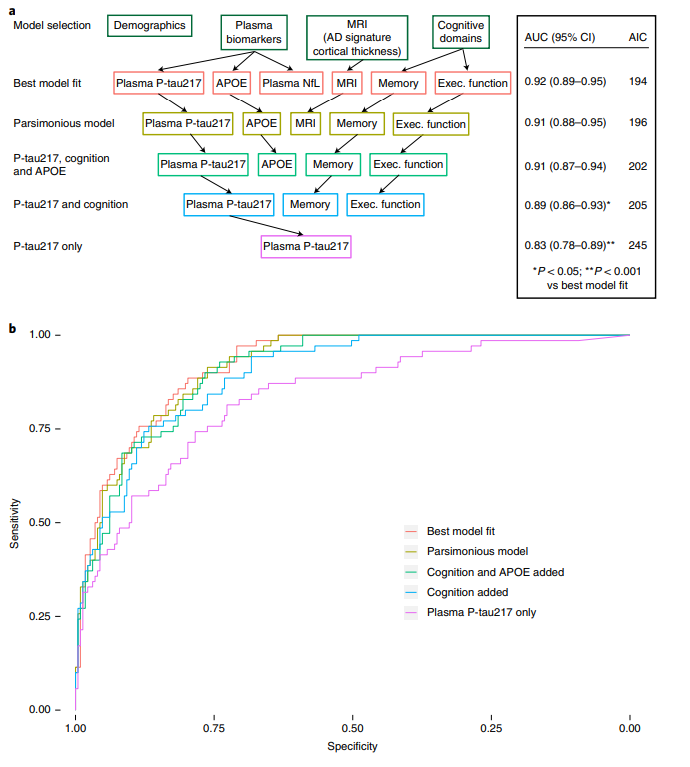
\includegraphics[height=18cm]{pic/AD217.PNG}}
	\caption{P-tau217預測 4 年內 AD圖}

	\label{fig:AD217}
\end{figure}
最佳模型為包括預測因子血漿 P-tau217、APOE 等位基因、執行功能、記憶功能、磁共振成像(magnetic resonance imaging,MRI)和血漿 NfL.該模型的 AUC 為 92\%;去除血漿 NfL和MRI,準確度(AUC=91\%)。


\section{用P-tau181預測 4 年內 AD }
\begin{figure}[H]
	\centering
	\centerline{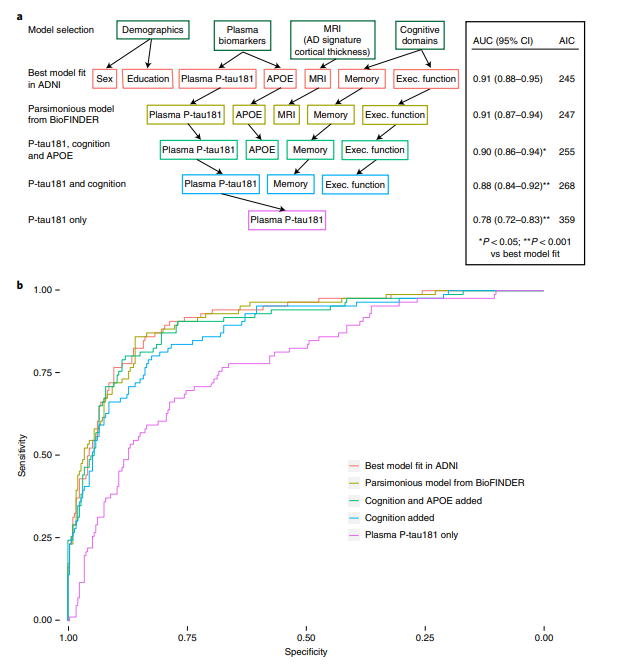
\includegraphics[height=18cm]{pic/AD181.PNG}}
	\caption{P-tau181預測 4 年內 AD圖}

	\label{fig:AD181}
\end{figure}
最佳模型為包括預測因子血漿 P-tau181、APOE 等位基因、執行功能、記憶功能、MRI,該模型的 AUC為91\%);去除MRI,準確度也還有(AUC = 90\%)。


\section{血漿用於預測AD結論}
預測主要在 4 年內進展為 AD 癡呆,雖然單獨血漿 P-tau217 可以在 4 年內準確預測 AD 癡呆(AUC = 83\%),但當它與APOE 基因型和認知測試相結合時,準確性的提高為顯著(AUC = 91\%)。就算加入能最為準確預測AD的MRI準確性的提高也只有而已(AUC = 92\%)。

使用血液的生物標誌,能避免運用MRI與脊髓抽取等對人體清害較大的方法進行AD的預測檢驗,只要進行抽血並配合執行力與記憶力功能等認知測驗,也能擁有寮好的的預測結果,幫助醫生在臨床上進行診斷。

\section{Reference}

Palmqvist S, Tideman P, Cullen N, Zetterberg H, Blennow K; Alzheimer’s Disease Neuroimaging Initiative, Dage JL, Stomrud E, Janelidze S, Mattsson-Carlgren N, Hansson O. Prediction of future Alzheimer's disease dementia using plasma phospho-tau combined with other accessible measures. Nat Med. 2021 Jun;27(6):1034-1042. doi: 10.1038/s41591-021-01348-z. Epub 2021 May 24. PMID: 34031605
%%ADEvaluate

\chapter{失智症之認知功能評估}
\label{chapter:intro}


\begin{figure}[H]
	\centering
	\centerline{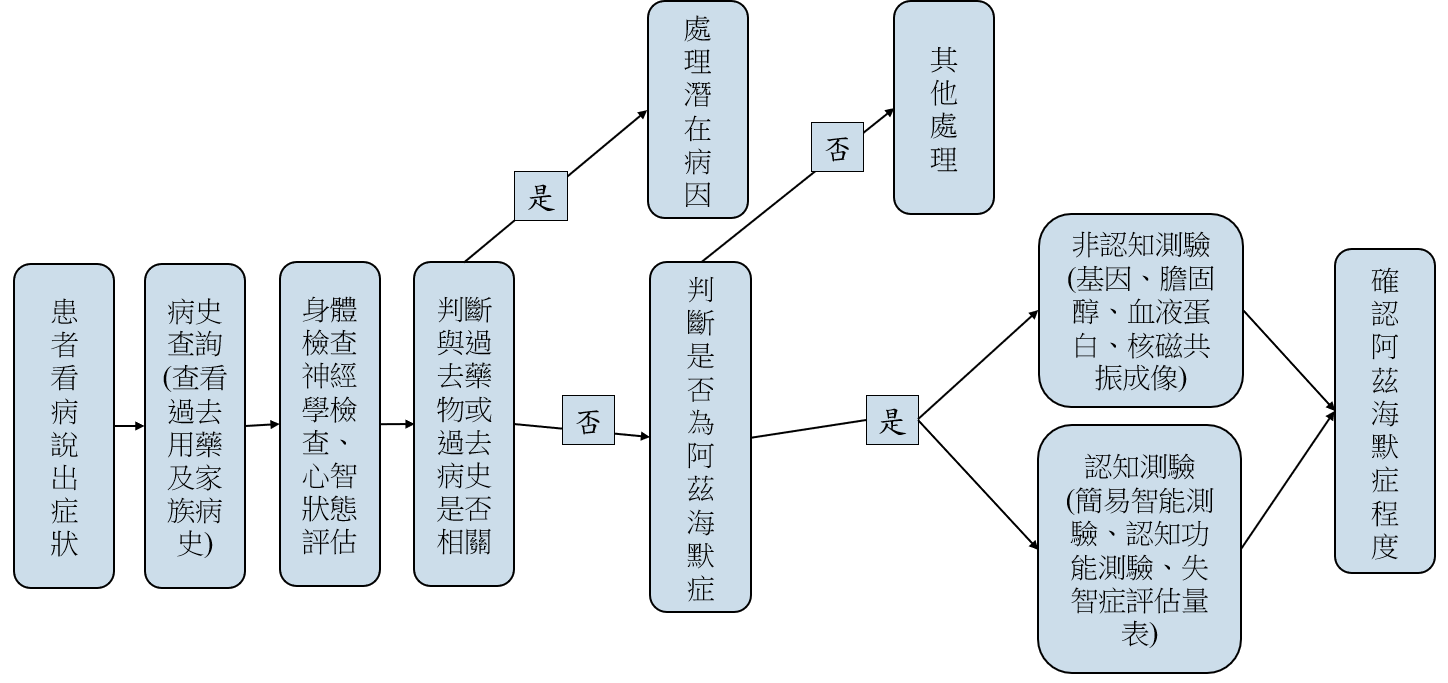
\includegraphics[height=8cm]{pic/ADprocess.PNG}}
	\label{fig:ADProcess}
\end{figure}
臨床數據集到的病人資料,包含性別、年齡、身高、體重、教育、飯前血糖(GLU-AC)、丙胺酸轉胺酶(GPT-ALT)、血清尿素濃度(Uric acid) 、肌酸酐(Creatinine) 、總膽固醇(CHOL-T)、三酸甘油酯(TG)、高密度脂蛋白(HDL-C)、低密度脂蛋白(LDL-C)、糖化血色素(HBA1C)、脂蛋白酶元E分型(APOE)、血管收縮素轉換酶(ACE)、基因型腦神經滋養因子(BDNF)、簡易智能測驗(MMSE)、認知功能障礙篩檢量表(CASI)、臨床失智症量表(CDR)等資料。簡易智能測驗(MMSE)、認知功能障礙篩檢量表(CASI)、臨床失智症量表(CDR)。

\section{臨床失智評估表(Clinical Dementia Rating,CDR)}

具有輕微認知症狀(例如記憶力下降)的患者是否患有前期或臨床前阿茲海默氏病(Alzheimer disease,AD)並在不久的將來發展為 AD 癡呆仍然是臨床醫生面臨的挑戰。這項任務對於正確和早期的 AD 診斷、開始對AD症治療、規劃未來以及希望很快開始改善疾病的治療都至關重要。

美國華盛頓大學的Hughes等人提出,用來評估阿茲海默 症患者日常生活及認知功能作整體性評估的量表。
用來對阿茲海默症患者,日常生活與認知功能作整體性評估的量表,是評估失智症嚴重程度的主要工具。隨著病程變化,某些特定日常生活功能會先出現障礙,當病程逐漸變嚴重時,其他不同日常生活障礙也陸續出現。藉由區分患者日常生活與認知功能障礙的程度,作為判定阿茲海默症嚴重程度的依據。


CDR包含有6個功能項目:
記憶力(為主要分數,M)、定向力、判斷與解決問題、社區事務、家居與嗜好、個人照料
對上述的6個功能項目,分為0到3總共5個不同功能程度。

\begin{itemize}
    \item
    0 代表健康 (Health)
    \item
    0.5 代表疑似或輕微障礙 (Questionable)
    \item
    1 代表輕度障礙 (Mild)
    \item
    2 代表中度障礙 (Moderate)
    \item
    3 代表重度障礙 (Severe)
\end{itemize}

分數判斷原則:
\begin{enumerate}
\item
若三個或以上的次要分數等於主要分數M(記憶力),則CDR的分數為M的分數。
\item
若三個次要分數在M的大於,而二個次要分數在M的小於,則CDR的分數為M的分數。
\item
若三個次要分數在M的小於,而二個次要分數在M的大於,則CDR的分數為M的分數。
\item
若過半數次要分數所在無法決定,則選最近M的分數。
\end{enumerate}

CDR是一個半結構性晤談的評估,主要包括兩個部份:
\begin{enumerate}
	\item
受試者部份:針對各種認知功能範圍,包括有注意力、長期記憶、近期記憶、時空定向力、語言、抽象與判斷等作評估。
\item
家人部份:詢問患者家人或主要照顧者,就受試者在日常生活上,是否有出現與記憶力有關的問題或困擾。
\end{enumerate}

\begin{figure}[H]
	\centering
	\centerline{\includegraphics[height=20cm]{pic/CDR.PNG}}
	\caption{CDR 臨床失智評分量表}
	\begin{minipage}{.7\linewidth}

		\footnotesize
		\emph{來源:}衛生福利部,失智症診療手冊

	\end{minipage}
	\label{fig:CDR}
\end{figure}

\section{簡易智能評估(Mini-Mental State Examination,MMSE)}
為臨床上最廣泛應用評估老年人認知狀態之工具,共分為定向感、記錄能力、注意力和計算力、回憶能力、抽象概念和語言能力來評估,滿分是三十分,答對一項給一分,若低於二十三分表度知能損傷,低於十六分表重度認知功能損傷。


是Folstein等人1975年所提出,2001年3月MMSE版權已轉為PAR, Inc.所有,任何臨床上使用、論文發表及研究使用需至PAR,Inc.網站申請版權使用。

MMSE (總分 30分) 包括五大施測項目 (下列括號中的數字為最高得分):
\begin{enumerate}
	\item
    定向感(10分):分為 時間定向力 (5分) 與 地點定向力 (5分) 兩部分。
	\item
	訊息登錄 (3分): 目的是要受試者學習三樣東西,稍後要作為短期回憶的測試使用。
	\item
	注意力與算術能力(5分):請受試者由 100 減 7 等於? 再減 7 等於?...連續進行五次。
	\item
    立即記憶與短期記憶(3分):詢問受試者是否記得先前重述的三樣東西 (順序無所謂)。
	\item
	語言理解、空間概念、與操作能力 (9分): 
	
	包含下列的問題:
	\begin{itemize}
		\item
		兩個一般常用物品的命名 (2分)。
		\item
		請受試者重述一個句子 (1分)。
		\item
		請受試者讀 “請閉上眼睛” 並做出動作(1分)。
		\item
		請受試者造一個句子並把它寫出來 (1分)。
		\item
		請受試者抄繪兩個五邊型其交叉為四邊型的圖形 (1分)。 
		\item
		請受試者在聽完 “用你的左手來拿這張紙,將它對折一半,然後交還給我” 的題目
後依序做出動作 (3分)。
	\end{itemize}

\end{enumerate}




\section{神經心理衡鑑(CASI)}
認知功能障礙篩檢量表 (CASI):經由固定的換算方式可以把它化成9個認知功能的細項,分別是長期記憶、注意力、時空定向力、語言能力、思緒流暢度、近期記憶、集中與心算力、抽象與判斷、空間概念
與構圖。

測驗總分100分,也可用於推估MMSE分數,MMSE施測的重要事項也可應用於CASI施測,CAIS會受教育程度與年齡影響。





%\section{附錄:MMSE和CDR}

%\includepdf[pages={1,2,3,4,5,6,7,8,9,10,11}]{MMSE.pdf}

%\includepdf[pages={1,2,3,4,5,6,7,8}]{CDR.pdf}

%%ReminiscenceTherapy
\chapter{Reminiscence Therapy[2]}
\label{chapter:intro}
\section{回憶療法(reminiscence therapy)介紹}
回憶療法,它涉及回憶和重新體驗老年人的生活事件,這種形式的治療干預個人的生活和經歷,意旨在幫助患者保持良好的心理健康。

回憶療法的兩個主要優點:改善認知功能和提高生活質量,以改善情緒和增強幸福、情緒為中心。不同的方法在研究中使用回憶療法來喚起故事、記憶和經歷。這意味著將患者的個人生活經歷作為分享的主題,同時展示照片、視頻和音樂等讓個人記憶深刻的具體對象。該療法對患者的認知、抑鬱、日常生活活動和生活質量均有顯著改善。回憶療法有效的重要因素是使用患者自己的生活故事和記憶。

\section{回憶療法操作}
至少每週一次,持續時間 30 至 60 分鐘或平均 45 分鐘,執行8到12週的時間,使用與患者過去經歷相關的高度刺激的具體對象,例如照片、視頻、音樂、患者過去的生活、記憶和經歷,可能對阿爾茨海默病患者產生最有益的影響。




%%  文獻
%\bibliographystyle{IEEEtran}
%    \bibliographystyle{plain}
%    \bibliographystyle{apa}
%    \bibliographystyle{apacite}\renewcommand{\bibname}{參考文獻}
%\bibliography{citations/ref_title1,citations/ref_title2}

%%%%%%%%%%%%%%%%---------- 附錄
%\begin{appendices}
%	\appendix
%	%        \noappendicestocpagenum
%	\titleformat{\chapter}[display]{\center\LARGE\sf}{附錄 \thechapter}{0.2cm}{}  % 設計附錄標題式樣,標題置中
%	\chapter{相關公式}
\label{chapter:appendix_eq}

    質能互換公式為\eqref{eq:mass_energy_equivalence}。
    \begin{equation}\label{eq:mass_energy_equivalence}
      E=MC^2
    \end{equation}

 %% appendix-A
%	\chapter{相關表格}
\label{chapter:appendix_tables}

    ○○○對應表為\ref{tab:mytitle2}。
    \begin{table}[htbp]
        \centering
        \caption{表格標題2}
        \label{tab:mytitle2}
        % Table generated by Excel2LaTeX from sheet '工作表1'
\begin{tabular}{rrr}
\toprule
Number & Class & Values \\
\midrule
1     & A     & 21 \\
2     & B     & 854 \\
3     & C     & 458 \\
4     & D     & 87 \\
5     & E     & 1654 \\
6     & F     & 978 \\
7     & G     & 23 \\
8     & H     & 746 \\
9     & I     & 278 \\
\bottomrule
\end{tabular}%

    \end{table}

 %% appendix-A
%\end{appendices}

%===============================================================
\end{document}
